% -*- coding: utf-8 -*-
\newpage
\section{Machine Learning}

Moving beyond traditional theoretical physical chemistry, this section explores
the rapidly evolving domain of Artificial Intelligence (\gls{AI}), with a
specific emphasis on Machine Learning (\gls{ML}). Although frequently perceived
as a recent innovation, \gls{AI} has undergone steady and significant
development over several decades~\cite{RussellNorvig2010}. Its applications now
range from personalised recommendations and autonomous driving to enabling
sophisticated language models capable of generating human-like
text~\cite{LeCun2015,Silver2016}. A notable recent advancement is the
introduction of attention mechanisms, exemplified by the Transformer
Architecture, which has dramatically reshaped fields such as natural language
processing and computer vision~\cite{Vaswani2017}.

\vspace{1em}%
Machine Learning, a subfield of \gls{AI}, focuses on algorithms capable of
learning patterns directly from data without explicit programming. This
paradigm broadly divides into: $i$) supervised learning ---where models learn
from labelled examples--- and $ii$) unsupervised learning ---which identifies
inherent structures within unlabelled data---. The algorithms go from
decision trees, and support vector machines (\gls{SVM}) to artificial neural
networks, each suited to distinct types of learning problems and
datasets~\cite{Goodfellow2016,Hastie2009} and they offer distinct trade-offs in
interpretability, computational complexity, and predictive
accuracy~\cite{Murphy2012,Bishop2006}.

\vspace{1em}%
In supervised learning, the objective is to predict outcomes based on
previously observed input-output pairs. Typical supervised learning tasks
encompass classification ---assigning data points to discrete categories--- and
regression-predicting continuous numerical values. Conversely, unsupervised
learning aims to uncover latent patterns or groupings within datasets lacking
predefined labels. Methods such as $k$-means clustering~\cite{Lloyd1982} and
hierarchical clustering~\cite{Johnson1967} illustrate this approach, seeking
natural groupings based purely on data similarity.

\newpage
\subsection{Preprocessing and Core Algorithms}

Data preprocessing significantly influences the success of \gls{ML} workflows.
Typically, raw data require cleaning, normalisation, and transformation steps
to handle inconsistencies, missing values, and outliers effectively. Feature
selection, identifying the most informative attributes, not only enhances model
performance but also simplifies model complexity, facilitating interpretability
and reducing computational overhead~\cite{Guyon2003}. Effective preprocessing
thus ensures that subsequent learning algorithms receive optimal input,
maximising predictive reliability and efficiency.

\vspace{1em}%
Neural networks, initially inspired by biological neurons~\cite{McCulloch1943},
have evolved significantly into complex, multilayered architectures known as
deep neural networks~\cite{LeCun2015}. Deep learning techniques have notably
driven breakthroughs in diverse domains, including image recognition, natural
language processing, and predictive modelling across scientific
disciplines~\cite{Krizhevsky2017,He2016}. Their capacity to model intricate,
nonlinear relationships within large-scale data makes neural networks
particularly valuable in chemistry, facilitating sophisticated predictive
models and augmenting traditional computational methodologies.

\vspace{1em}%
Decision trees provide intuitive and interpretable models by segmenting data
into homogeneous subsets based on feature values~\cite{Quinlan1986}. Support
Vector Machines, introduced by Cortes and Vapnik~\cite{Cortes1995}, offer
powerful classification capabilities by determining optimal hyperplanes that
maximise class separation margins. \glspl{SVM} effectively handle linear and
nonlinear problems through kernel functions, transforming inputs implicitly
into higher-dimensional feature spaces~\cite{Scholkopf2002}. This flexibility
allows \glspl{SVM} to robustly classify complex data distributions that may not
be linearly separable in their original dimensionality.

\newpage

\subsection{Classifying Data with Machine Learning}

Clustering is a common task in supervised and unsupervised \gls{ML}, aiming to
group data into subsets (clusters) such that data points within a cluster share
similar characteristics. One of the most widely used clustering algorithms is
$k$-means~\cite{Lloyd1982}, which partitions a dataset into $k$ clusters by
iteratively assigning each point to the nearest cluster centroid and
recomputing the centroids to minimise intra-cluster variance.

% Despite its efficiency and simplicity, $k$-means assumes spherical cluster
% shapes and is sensitive to initialisation, which may lead to suboptimal
% convergence.

% Formaly, for a given a set of $n$ observations $\{\mathbf{x}_1, \dots, \mathbf{x}_n\} \subset
% \rreal[d]$, $k$-means clustering aims to partition the data into $k$ disjoint
% clusters $S = \{S_1, \dots, S_k\}$ such that the within-cluster sum of squares
% is minimised; the objective function is

% \begin{align}
%   \underset{S}{\arg\min} \sum_{i=1}^{k} \sum_{\mathbf{x} \in S_i}
%   \|\mathbf{x} - \boldsymbol{\mu}_i\|^2.
% \end{align}

% \noindent where $\boldsymbol{\mu}_i$ denotes the centroid of cluster $S_i$,
% computed as the mean of the points assigned to it. The algorithm proceeds
% iteratively: initial centroids are selected (often randomly), each point is
% assigned to the nearest centroid, centroids are recomputed, and the process
% repeats until convergence. While the optimisation problem is NP-hard in
% general, Lloyd's algorithm~\cite{Lloyd1982} provides an efficient heuristic
% that converges to a local minimum. Despite its simplicity, the method's
% performance depends heavily on the initialisation and the choice of $k$, which
% must typically be determined using domain knowledge or validation techniques
% such as the silhouette score or elbow method.

An alternative approach that overcomes some of these limitations is the Support
Vector Clustering (\gls{SVC}), derived from \gls{SVM}, \gls{SVC} maps the data
into a high-dimensional feature space using a kernel function, ---typically the
radial basis function (RBF) kernel---, and
constructs a minimal enclosing hypersphere~\cite{BenHur2001}. The pre-image of
this hypersphere in input space forms cluster boundaries, allowing the method
to capture non-convex structures that are inaccessible to centroid-based
techniques. The \texttt{scikit-learn} implementation of \gls{SVC} provides practical
access to this method, with straightforward interfaces for adjusting the kernel
and its parameters, such as the parameter $C$~\cite{scikit-learn}.

Formaly, let $\phi: \rreal[n] \rightarrow \mathcal{F}$ be a nonlinear mapping from the
input space to a high-dimensional feature space $\mathcal{F}$. In this
transformed space, \gls{SVC} constructs the smallest enclosing sphere by
solving the following optimisation problem:
%
\begin{align}
  \min_{\mathbf{a}, R, \xi_i} \quad R^2 + C \sum_{i=1}^N \xi_i \quad \text{subject to} \quad
  \|\phi(\mathbf{x}_i) - \mathbf{a}\|^2 \leq R^2 + \xi_i,\quad \xi_i \geq 0.
\end{align}

\noindent where, $\mathbf{a}$ is the centre of the sphere, $R$ its radius, and
$C > 0$ is a regularisation parameter that controls the trade-off between the
tightness of the boundary and the tolerance to outliers.

The use of the kernel trick enables this problem to be solved without explicit
knowledge of $\phi$, relying only on kernel evaluations $K(\mathbf{x}_i,
\mathbf{x}_j) = \langle \phi(\mathbf{x}_i), \phi(\mathbf{x}_j) \rangle$.

The choice of kernel function $K(\mathbf{x}, \mathbf{x}')$ is central to the
flexibility and performance of \gls{SVC}. The kernel implicitly
defines the geometry of the feature space and, consequently, the shape of the
cluster boundaries. Some commonly used kernels include:

\newpage
\begin{itemize}
  \item \textbf{Linear kernel}:
    $K(\mathbf{x}, \mathbf{x}') = \mathbf{x}^\top \mathbf{x}'$
    Equivalent to no transformation; effective when data are linearly separable.

  \item \textbf{Polynomial kernel}:
    $K(\mathbf{x}, \mathbf{x}') = (\gamma \mathbf{x}^\top \mathbf{x}' + r)^d$
    Introduces interactions up to degree $d$; parameters $\gamma > 0$,
    $r \in \rreal$, and $d \in \nnatural$ control flexibility and curvature.

  \item \textbf{Radial Basis Function (RBF) kernel}:
    $K(\mathbf{x}, \mathbf{x}') = \exp(-\gamma \|\mathbf{x} - \mathbf{x}'\|^2)$
    Maps input to an infinite-dimensional feature space. Suitable for
    nonlinearly separable data; parameter $\gamma > 0$ controls the
    radius of influence of support vectors.

  \item \textbf{Sigmoid kernel}:
    $K(\mathbf{x}, \mathbf{x}') = \tanh(\gamma \mathbf{x}^\top \mathbf{x}' + r)$
    Related to neural networks; behaves like a two-layer perceptron.
    Less commonly used due to non-positive definiteness for some parameters.

\end{itemize}

\begin{figure}[H]
  \centering
  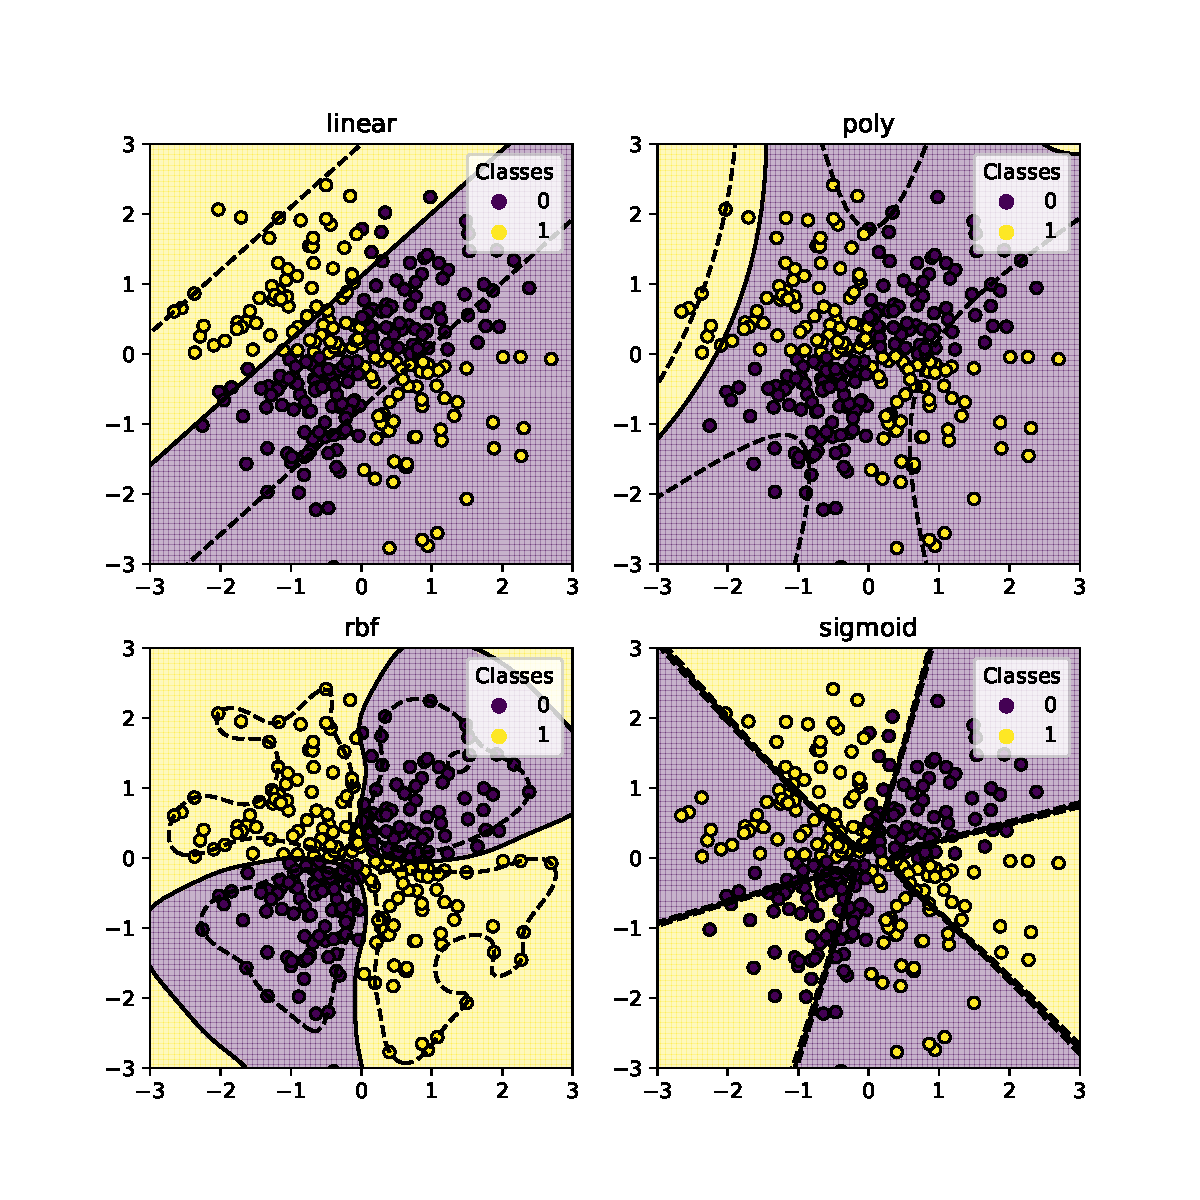
\includegraphics[width=0.81\textwidth]{img/kernels}
  \caption{Visualisation of different kernel functions in SVC. The plot shows
    the decision boundaries formed by each kernel on a synthetic dataset with
    two classes. Data taken from the \texttt{scikit-learn}
    documentation~\cite{scikit-svm-kernels}.}
  \label{plot_kernels}
\end{figure}

% \newpage
The RBF kernel is the default and most widely used option in unsupervised SVC
applications, as it allows capturing highly nonlinear and non-convex cluster
structures with smooth boundaries. In the Figure~\ref{plot_kernels}, we
illustrate the effect of different kernels, note that the plots do not evaluate
the kernel's accuracy, they only provide a visual understanding.

\subsection{Predicting Numerical Values with Machine Learning}

In supervised machine learning, regression models aim to predict continuous
numerical quantities from structured input features. This capability is
particularly useful in theoretical and computational chemistry, where properties
such as reactivity indices, energies, or solvation parameters can be modelled
from molecular descriptors without requiring the full cost of ab initio
calculations. A variety of regression algorithms exist, each making different
assumptions about the data and offering different trade-offs between accuracy,
interpretability, and computational efficiency.

Ensemble methods, such as Random Forest Regression (RFR), are among the most
widely used approaches. RFR builds an ensemble of
decision trees~\cite{Breiman2001}, each trained on a bootstrap sample of the
data and employing random subsets of features to reduce variance and prevent
overfitting. The final prediction is obtained by averaging the outputs of the
individual trees. Random Forests offer high accuracy with minimal tuning and
handle nonlinear interactions and mixed-type features effectively, which makes
them well suited to heterogeneous chemical datasets.

Artificial neural networks (ANNs), and in particular deep architectures, can
approximate complex nonlinear functions and are capable of capturing subtle
patterns in the input data~\cite{Goodfellow2016}. A feedforward neural network
comprises layers of nodes (neurons), each applying an affine transformation
followed by a nonlinear activation function. When properly regularised and
trained on sufficient data, ANNs can generalise well to unseen examples.
However, they often require careful hyperparameter tuning and are sensitive to
overfitting, particularly in low-data regimes, and commonly require large
datasets to achieve optimal performance.

\newpage
Alternative probabilistic regression models include Bayesian Ridge Regression
(BRR) and Gaussian Process Regression (GPR). BRR extends classical linear
regression by placing Gaussian priors on the coefficients, yielding a
Bayesian posterior that reflects uncertainty over predictions~\cite{Tipping2001}.
In contrast, GPR is a nonparametric method that models the output as a
realisation of a Gaussian process~\cite{Rasmussen2006}, fully defined by a mean
function and covariance kernel. GPR provides both point estimates and
predictive uncertainty, making it appealing in scientific
applications where uncertainty quantification is essential.


